 % mainfile: ../../../../master.tex
\subsection{Conduct Experiments on AOSP 14}
\label{task:20240213_aosp}

\subsubsection{Mine Permission Mappings for AOSP 14}

Set up Java and compile the Java code:
\begin{lstlisting}
sudo apt install openjdk-8-jdk-headless   # version 8u382-ga-1ubuntu1
rm -rf out && mkdir out && javac src/*.java src/javaLink/*.java src/cppLink/*.java src/util/*.java -cp "./libs/*" -d out && java -cp "./out:./libs/*" findJavaLink
sudo update-alternatives --config java
\end{lstlisting}

Gets error message:
\begin{lstlisting}
Exception in thread "main" java.lang.RuntimeException: java.util.concurrent.ExecutionException: java.lang.Exception: Error: The path '/Library/Java/JavaVirtualMachines/jdk1.8.0_231.jdk/Contents/Home/jre/lib/rt.jar' does not exist.
    at soot.SourceLocator.getClassSourceType(SourceLocator.java:312)
    at soot.SourceLocator.lookupInClassPath(SourceLocator.java:615)
    at soot.asm.AsmClassProvider.find(AsmClassProvider.java:39)
    at soot.SourceLocator.getClassSource(SourceLocator.java:187)
    at soot.SootResolver.bringToHierarchyUnchecked(SootResolver.java:231)
    at soot.SootResolver.bringToHierarchy(SootResolver.java:221)
    at soot.SootResolver.bringToSignatures(SootResolver.java:292)
    at soot.SootResolver.bringToBodies(SootResolver.java:332)
    at soot.SootResolver.processResolveWorklist(SootResolver.java:171)
    at soot.SootResolver.resolveClass(SootResolver.java:141)
    at soot.Scene.forceResolve(Scene.java:2095)
    at javaLink.JavaLink.run(JavaLink.java:78)
    at findJavaLink.main(findJavaLink.java:14)
Caused by: java.util.concurrent.ExecutionException: java.lang.Exception: Error: The path '/Library/Java/JavaVirtualMachines/jdk1.8.0_231.jdk/Contents/Home/jre/lib/rt.jar' does not exist.
    at com.google.common.util.concurrent.AbstractFuture.getDoneValue(AbstractFuture.java:552)
    at com.google.common.util.concurrent.AbstractFuture.get(AbstractFuture.java:513)
    at com.google.common.util.concurrent.AbstractFuture$TrustedFuture.get(AbstractFuture.java:90)
    at com.google.common.util.concurrent.Uninterruptibles.getUninterruptibly(Uninterruptibles.java:197)
    at com.google.common.cache.LocalCache$Segment.getAndRecordStats(LocalCache.java:2229)
    at com.google.common.cache.LocalCache$Segment.loadSync(LocalCache.java:2195)
    at com.google.common.cache.LocalCache$Segment.lockedGetOrLoad(LocalCache.java:2153)
    at com.google.common.cache.LocalCache$Segment.get(LocalCache.java:2043)
    at com.google.common.cache.LocalCache.get(LocalCache.java:3851)
    at com.google.common.cache.LocalCache.getOrLoad(LocalCache.java:3875)
    at com.google.common.cache.LocalCache$LocalLoadingCache.get(LocalCache.java:4800)
    at soot.SourceLocator.getClassSourceType(SourceLocator.java:310)
    ... 12 more
Caused by: java.lang.Exception: Error: The path '/Library/Java/JavaVirtualMachines/jdk1.8.0_231.jdk/Contents/Home/jre/lib/rt.jar' does not exist.
    at soot.SourceLocator$1.load(SourceLocator.java:73)
    at soot.SourceLocator$1.load(SourceLocator.java:68)
    at com.google.common.cache.LocalCache$LoadingValueReference.loadFuture(LocalCache.java:3445)
    at com.google.common.cache.LocalCache$Segment.loadSync(LocalCache.java:2194)
    ... 18 more
\end{lstlisting}

So, find the available Java libraries in our machine using \texttt{sudo find / -iname rt.jar}:
\begin{lstlisting}
/home/weiminn/Documents/aosp13/prebuilts/jdk/jdk8/darwin-x86/jre/lib/rt.jar
/home/weiminn/Documents/aosp13/prebuilts/jdk/jdk8/linux-x86/jre/lib/rt.jar
/home/weiminn/Documents/aosp14/prebuilts/jdk/jdk8/darwin-x86/jre/lib/rt.jar
/home/weiminn/Documents/aosp14/prebuilts/jdk/jdk8/linux-x86/jre/lib/rt.jar
find: '/proc/1246576': No such file or directory
/usr/lib/jvm/java-8-openjdk-amd64/jre/lib/rt.jar
find: '/run/user/1000/gvfs': Permission denied
find: '/run/user/1000/doc': Permission denied
\end{lstlisting}

Change the following contents of \texttt{Config.java} to:
\begin{lstlisting}
//     static String MAC_jreDir = "/Library/Java/JavaVirtualMachines/jdk1.8.0_231.jdk/Contents/Home/jre/lib/rt.jar";
//     static String MAC_jceDir = "/Library/Java/JavaVirtualMachines/jdk1.8.0_231.jdk/Contents/Home/jre/lib/jce.jar";

static String MAC_jreDir = "/usr/lib/jvm/java-8-openjdk-amd64/jre/lib/rt.jar";
static String MAC_jceDir = "/usr/lib/jvm/java-8-openjdk-amd64/jre/lib/jce.jar";

//     static String MAC_ANDROID_JAR = "/android-hidden-api-master/android-26/android.jar";
//     static String MAC_SERVICES_JAR = "/android-hidden-api-master/android-26/services.jar";

static String MAC_ANDROID_JAR = "/home/weiminn/Android/Sdk/platforms/android-34/android.jar";
static String MAC_SERVICES_JAR = "/home/weiminn/Documents/aosp14/out/target/product/emulator_x86_64/system/framework/services.jar";
\end{lstlisting} 

Error message:
\begin{lstlisting}
Exception in thread "main" java.lang.RuntimeException: java.util.concurrent.ExecutionException: java.lang.Exception: Error: The path '/home/weiminn/Documents/NatiDroid/jar8.1/services.devicepolicy_intermediates.jar' does not exist.
    at soot.SourceLocator.getClassSourceType(SourceLocator.java:312)
    at soot.SourceLocator.lookupInClassPath(SourceLocator.java:615)
    at soot.asm.AsmClassProvider.find(AsmClassProvider.java:39)
    at soot.SourceLocator.getClassSource(SourceLocator.java:187)
    at soot.SootResolver.bringToHierarchyUnchecked(SootResolver.java:231)
    at soot.SootResolver.bringToHierarchy(SootResolver.java:221)
    at soot.SootResolver.bringToSignatures(SootResolver.java:292)
    at soot.SootResolver.bringToBodies(SootResolver.java:332)
    at soot.SootResolver.processResolveWorklist(SootResolver.java:171)
    at soot.SootResolver.resolveClass(SootResolver.java:141)
    at soot.Scene.forceResolve(Scene.java:2095)
    at javaLink.JavaLink.run(JavaLink.java:78)
    at findJavaLink.main(findJavaLink.java:14)
Caused by: java.util.concurrent.ExecutionException: java.lang.Exception: Error: The path '/home/weiminn/Documents/NatiDroid/jar8.1/services.devicepolicy_intermediates.jar' does not exist.
    at com.google.common.util.concurrent.AbstractFuture.getDoneValue(AbstractFuture.java:552)
    at com.google.common.util.concurrent.AbstractFuture.get(AbstractFuture.java:513)
    at com.google.common.util.concurrent.AbstractFuture$TrustedFuture.get(AbstractFuture.java:90)
    at com.google.common.util.concurrent.Uninterruptibles.getUninterruptibly(Uninterruptibles.java:197)
    at com.google.common.cache.LocalCache$Segment.getAndRecordStats(LocalCache.java:2229)
    at com.google.common.cache.LocalCache$Segment.loadSync(LocalCache.java:2195)
    at com.google.common.cache.LocalCache$Segment.lockedGetOrLoad(LocalCache.java:2153)
    at com.google.common.cache.LocalCache$Segment.get(LocalCache.java:2043)
    at com.google.common.cache.LocalCache.get(LocalCache.java:3851)
    at com.google.common.cache.LocalCache.getOrLoad(LocalCache.java:3875)
    at com.google.common.cache.LocalCache$LocalLoadingCache.get(LocalCache.java:4800)
    at soot.SourceLocator.getClassSourceType(SourceLocator.java:310)
    ... 12 more
Caused by: java.lang.Exception: Error: The path '/home/weiminn/Documents/NatiDroid/jar8.1/services.devicepolicy_intermediates.jar' does not exist.
    at soot.SourceLocator$1.load(SourceLocator.java:73)
    at soot.SourceLocator$1.load(SourceLocator.java:68)
    at com.google.common.cache.LocalCache$LoadingValueReference.loadFuture(LocalCache.java:3445)
    at com.google.common.cache.LocalCache$Segment.loadSync(LocalCache.java:2194)
    ... 18 more
\end{lstlisting}

Modify \path{/home/weiminn/Documents/NatiDroid/py/collect_jar.py}:
\begin{lstlisting}
version = '7.0'
project_path = '/android-7.0.0_r33/out/target/common/obj/JAVA_LIBRARIES'

version = '14.0'
project_path = '/home/weiminn/Documents/aosp14/out/target/common/obj/JAVA_LIBRARIES'
\end{lstlisting}

% \begin{longtable}{p{.5\linewidth}p{.25\linewidth}p{.25\linewidth}} 
% \toprule
% Step & File & Function \\
% \midrule
% \endhead

% Intermediate \texttt{.jar} files
% &\texttt{}
% &\texttt{}
% \\

% Extract build commands from \texttt{.ninja} file
% &\texttt{}
% &\texttt{}
% \\

% Merge ninja commands
% &\texttt{}
% &\texttt{}
% \\

% Replace Clang++ commands with Clang commands
% &\texttt{}
% &\texttt{}
% \\
% Identify AIDL communication using stub-proxy pattern
% &\texttt{}
% &\texttt{}
% \\

% Identify JNI communication by \texttt{RegisterMethodsOrDie},  \texttt{registerNativeMethods}, and  \texttt{jniRegisterNativeMethods}.
% &\texttt{}
% \\

% Forward analysis on the native side
% &\texttt{}
% \\

% Backward analysis on the Java side
% &\texttt{}
% \\

% Connect the two CFGs
% &\texttt{}
% \\

% Handle service identifier
% &\texttt{}
% \\

% Handle Android strong pointer
% &\texttt{}
% \\

% Handle member variable
% &\texttt{}
% \\

% Extract Protection Mapping using DFS
% &\texttt{}
% \\

% \midrule
% \caption{Permission Denied Syntax} 
% \label{tab:permissiondeniedsyntax}
% \end{longtable}


% 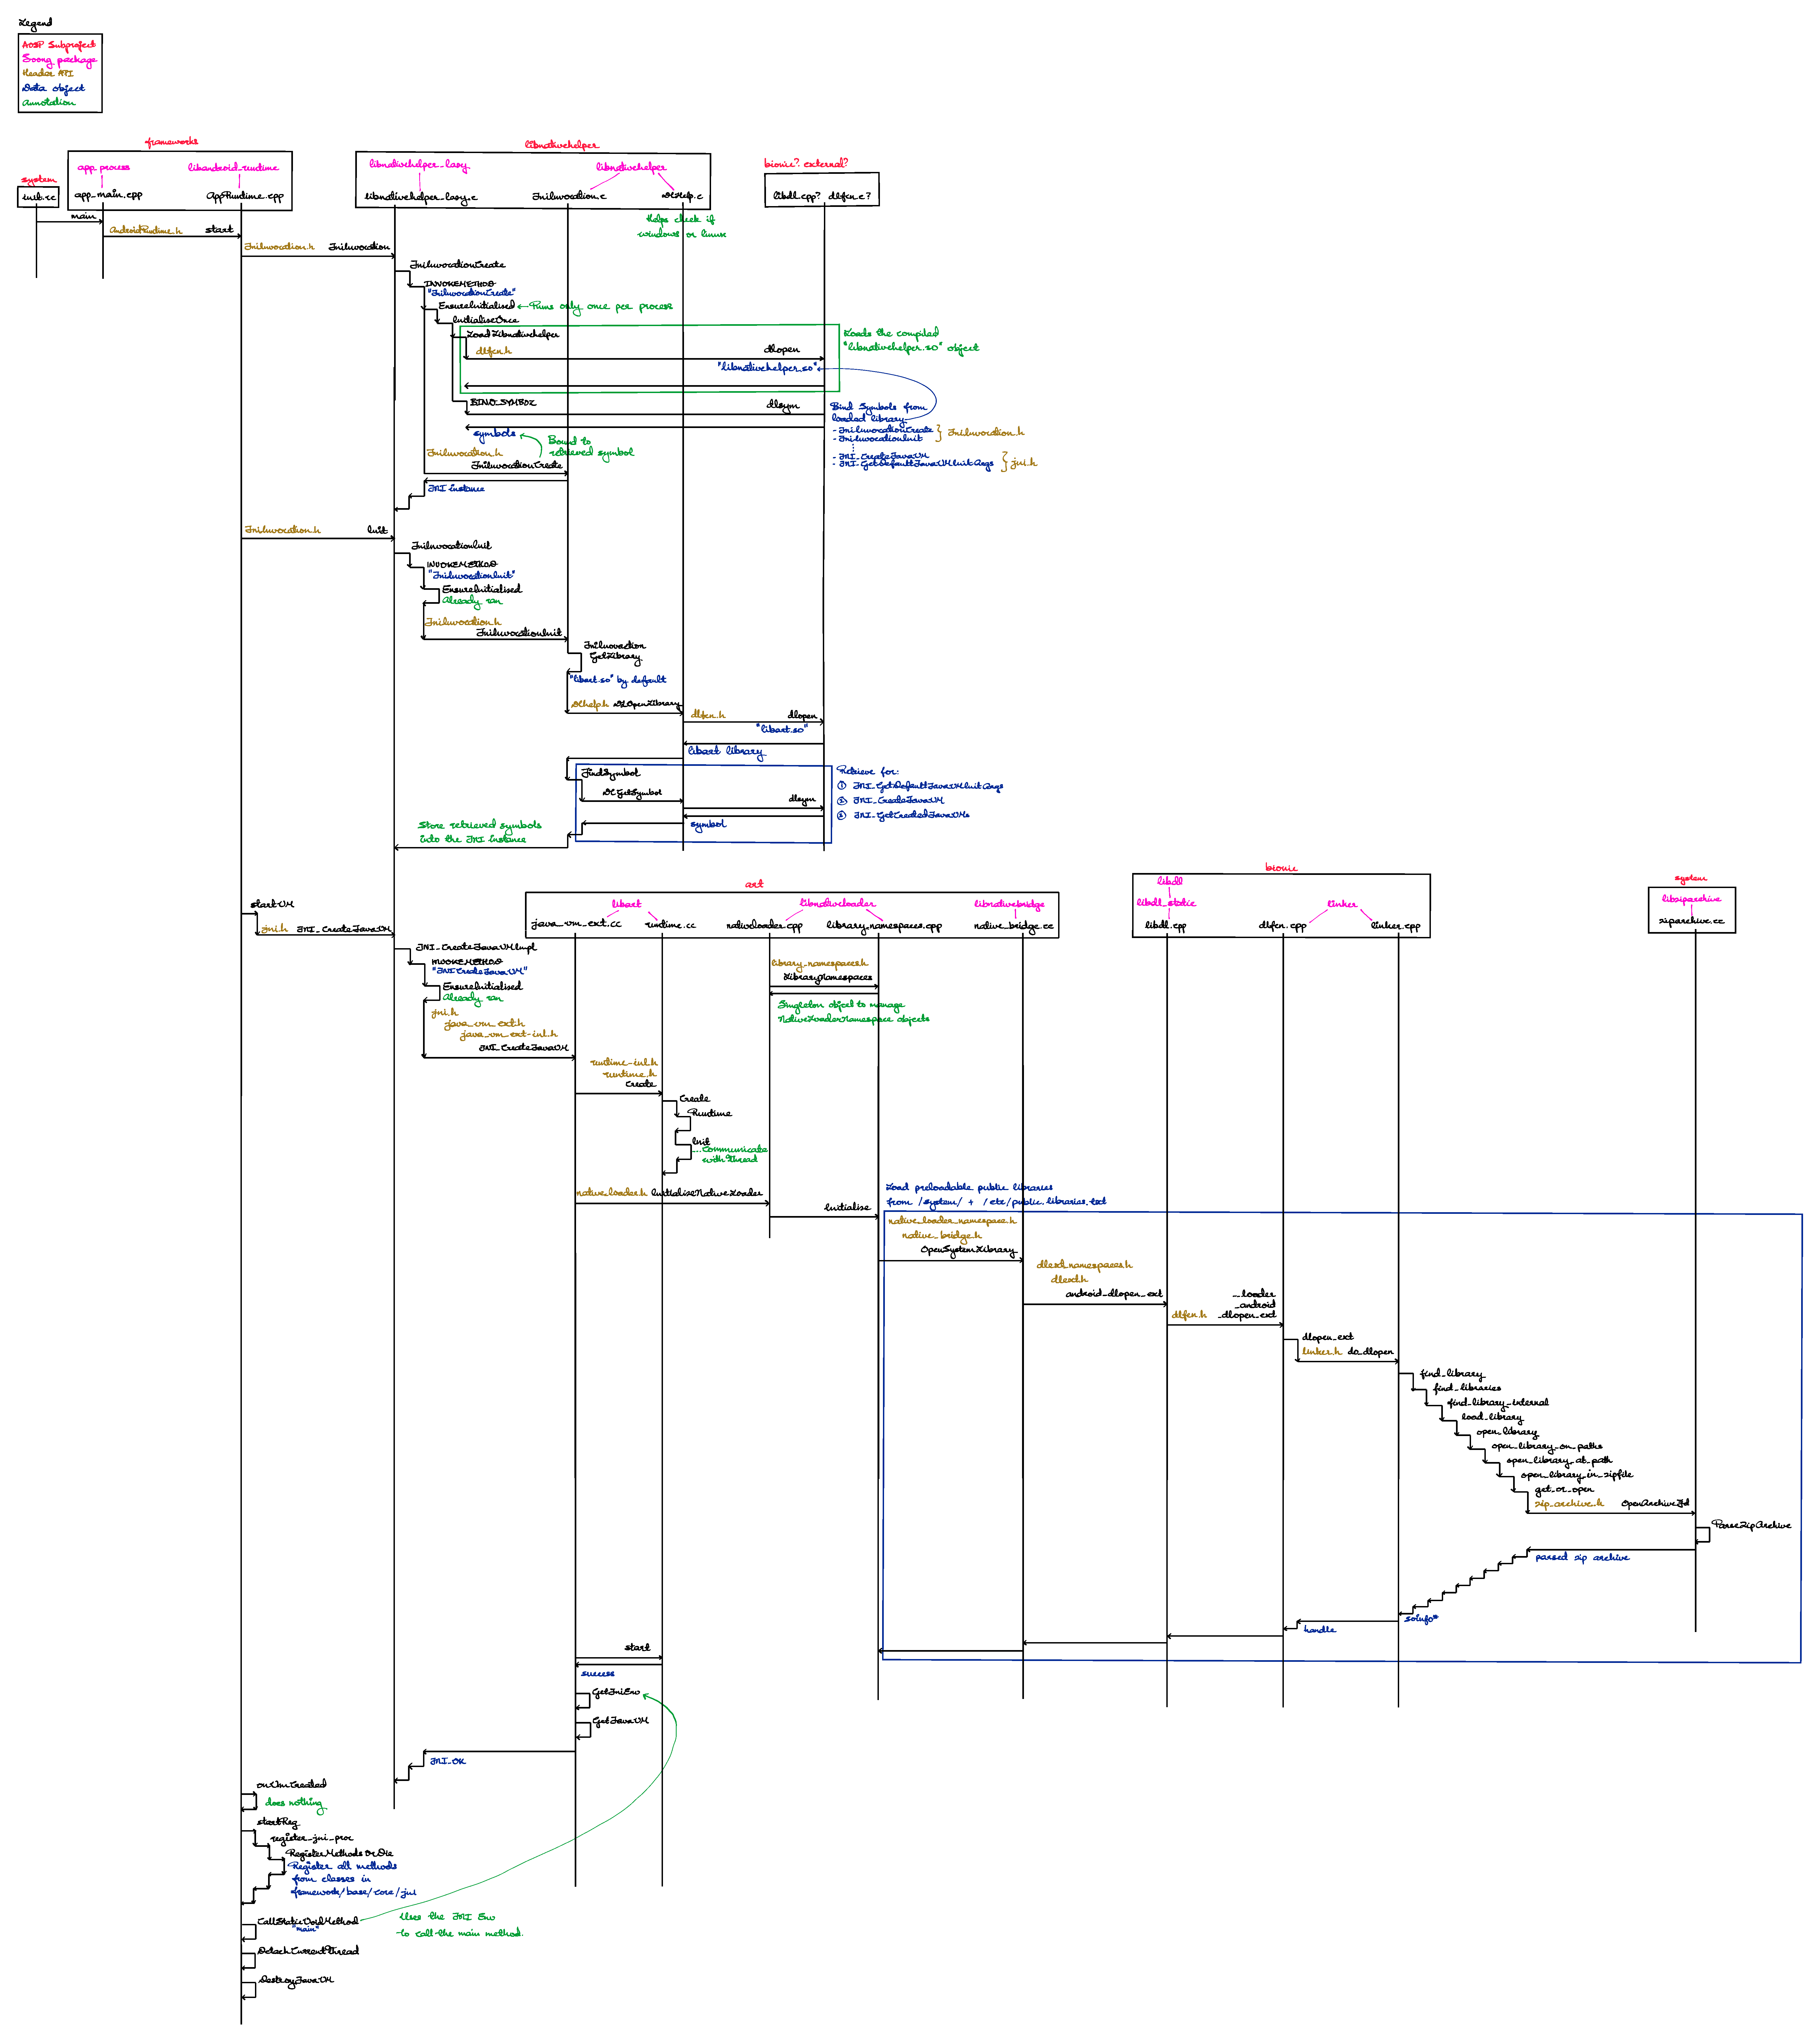
\includepdf[pages=-, scale=.95,pagecommand={}]{entries/2024/01/01/art.pdf}

% \begin{itemize}
% \item \textbf{Domain.} The context of the process that is acting upon something.
% \item \textbf{Type.} The context of the resource on which the process is acting.
% \item \textbf{Class.} The object class of the resource (e.g. \textit{file} or \textit{socket}).
% \item \textbf{Permissions.} The permissions that are allowed given the \textit{domain}, \textit{type} and \textit{class}.
% \end{itemize}

% SELinux rule syntax:
% \begin{lstlisting}
% allow <domain> <type>:<class> { <permissions> };
% \end{lstlisting}

% \subsubsection{Decoding Permission Denial Message}

% Message:
% \begin{lstlisting}
% type=AVC msg=audit(1363289005.532:184): avc:  denied  { read } for  pid=29199 comm="Trace" 
% name="online" dev="sysfs" ino=30 scontext=staff_u:staff_r:googletalk_plugin_t 
% tcontext=system_u:object_r:sysfs_t tclass=file
% \end{lstlisting}

% \begin{longtable}{p{.15\linewidth}p{.15\linewidth}p{.65\linewidth}} 
% \toprule
% Log part & Name & Description \\
% \midrule
% \endhead

% \texttt{ino=30}
% &inode number
% &The inode number of the target file. In this case, since we know it is on the \texttt{sysfs} file system, we can look for this file using: \texttt{find /sys -xdev -inum 30}
% \\

% \texttt{tclass=file}
% &Target class
% &The class of the target.
% \\

% \midrule
% \caption{Permission Denied Syntax} 
% \label{tab:permissiondeniedsyntax}
% \end{longtable}


% \subsubsection{SELinux Architecture}

% SELinux consists of four main components: object managers (OM), access vector cache (AVC), security server, and security policy as show below:
% \begin{figure}[H]
%     \centering
%     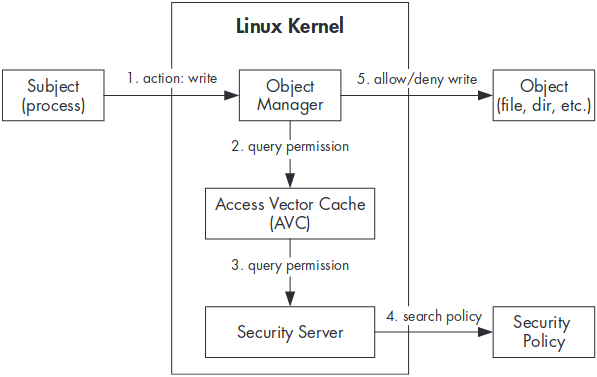
\includegraphics[width=.85\linewidth]{entries/2023/12/10/selinux.png}
%     \caption{SELinux Components}
%     \label{fig:selinux}
% \end{figure}
